\documentclass[10pt]{standalone}
\usepackage{tikz,my-tikz-clipart}


\begin{document}

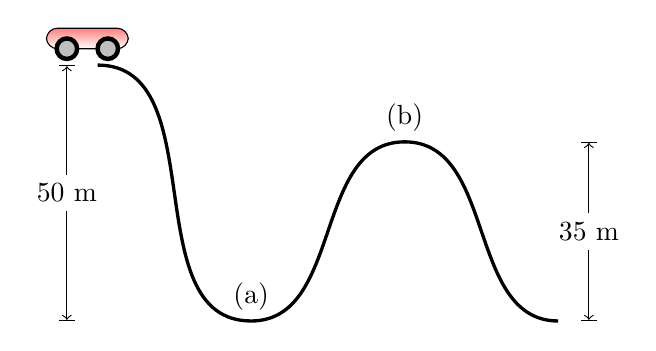
\begin{tikzpicture}[x=0.65cm, y=0.65cm]
  \def\xs{3}
  \draw[very thick] 
    (1*\xs,5) 
    to[in=180,out=0] (2*\xs,0) node[above] {(a)}
    to[in=180,out=0] (3*\xs,3.5) node[above] {(b)}
    to[in=180,out=0] (4*\xs,0);

  \draw[|<->|] (.8*\xs,0) -- (.8*\xs,5) 
    node[midway,fill=white] {50 m};
  \draw[|<->|] (4.2*\xs,0) -- (4.2*\xs,3.5) 
    node[midway,fill=white] {35 m};


  \begin{scope}[scale=0.4,shift={(5,13.3)}]
    \filldraw[top color=red!50, draw=black, rounded corners] 
      (0,0) -- (0,1) -- 
      (4,1) -- (4,0) -- cycle;
    \draw[fill=gray!50, draw=black, ultra thick] 
      (1,0) circle (.5);
    \draw[fill=gray!50, draw=black, ultra thick] 
      (3,0) circle (.5);
  \end{scope}
\end{tikzpicture}

\end{document}